% !TeX root = ../navier-stokes-manuscript.tex
\subsection{The perfectly stretching vortex}\label{sub:ThePerfectlyBalancedRipCordVortex}

Take one smooth vortex and stretch it along its axis. The fluid is incompressible, so the lengthening cannot happen alone: the cross-section narrows at the same time. The rotation is now packed into a smaller radius, the winding tightens, and the velocity changes more sharply as we move across the core. Stretch it again and the same thing happens again. Each stretch hands the next one a thinner vortex with steeper variation already in place.

Keep the vortex perfectly centred while this happens. Let no wobble carry it off axis, no buckling fold it away from the stretching direction, and no fragmentation break the core before the next stretch. This is the perfectly stretching vortex. It is a thought experiment, not a claim that we have written down an exact special solution. Its purpose is to give concentration every geometric advantage and leave the Navier--Stokes equation itself responsible for what happens next.

The word \emph{core} has two possible meanings here, and they cannot be mixed. The core may contain the same material particles throughout the narrowing. Or it may be a visible region that keeps recruiting new particles while earlier ones leave. The first reading is about the separation of fixed fluid labels. The second is about concentration in the complete velocity field. Both can look like the same tightening vortex, so we will carry both readings and close them separately.

\begin{center}
\captionsetup{hypcap=false}
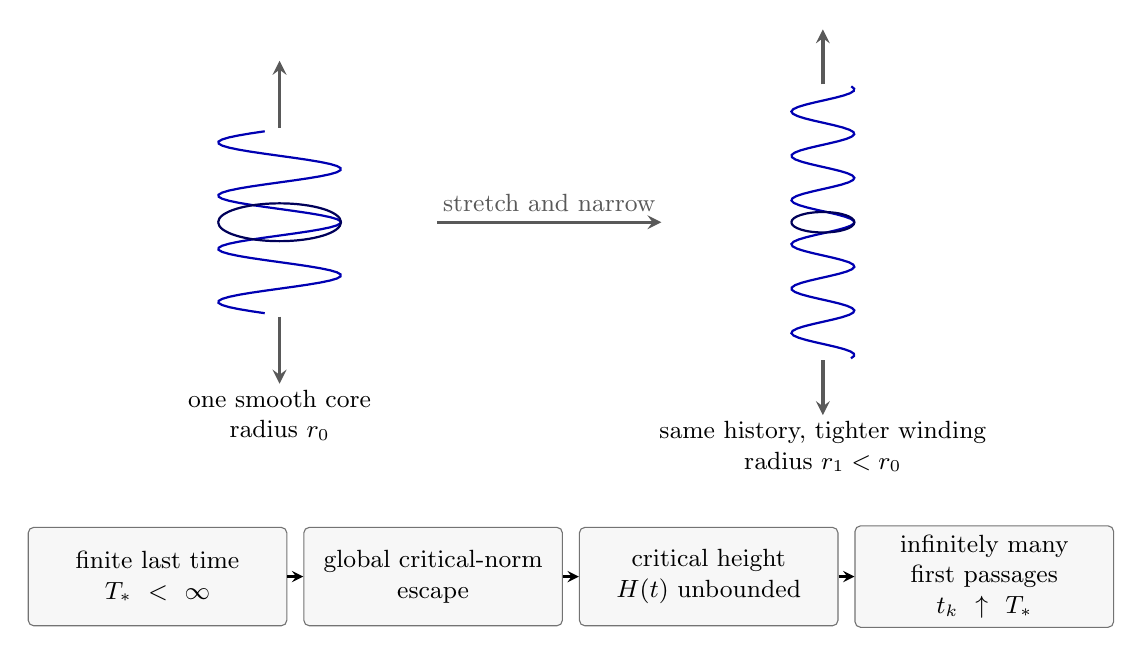
\begin{tikzpicture}[
  >=stealth,
  logic/.style={draw=black!55,rounded corners=2pt,fill=black!3,
    align=center,text width=3.05cm,minimum height=1.25cm,font=\small},
  note/.style={align=center,font=\small}
]
  \draw[blue!70!black,thick,domain=-1.1:1.1,samples=90]
    plot ({-3.7+0.78*cos(560*\x)},{1.05*\x+2.4});
  \draw[blue!35!black,thick] (-4.48,2.4) arc[start angle=180,end angle=540,x radius=.78,y radius=.24];
  \draw[->,very thick,black!65] (-3.7,3.6)--(-3.7,4.45);
  \draw[->,very thick,black!65] (-3.7,1.2)--(-3.7,.35);
  \node[note] at (-3.7,-.05) {one smooth core\\radius \(r_0\)};

  \draw[->,very thick,black!65] (-1.7,2.4)--(1.15,2.4)
    node[midway,above,note] {stretch and narrow};

  \draw[blue!70!black,thick,domain=-1.35:1.35,samples=120]
    plot ({3.2+0.40*cos(820*\x)},{1.28*\x+2.4});
  \draw[blue!35!black,thick] (2.80,2.4) arc[start angle=180,end angle=540,x radius=.40,y radius=.13];
  \draw[->,very thick,black!65] (3.2,4.15)--(3.2,4.85);
  \draw[->,very thick,black!65] (3.2,.65)--(3.2,-.05);
  \node[note] at (3.2,-.45) {same history, tighter winding\\radius \(r_1<r_0\)};

  \node[logic] (a) at (-5.25,-2.1) {finite last time\\\(T_*<\infty\)};
  \node[logic] (b) at (-1.75,-2.1) {global critical-norm\\escape};
  \node[logic] (c) at (1.75,-2.1) {critical height\\\(H(t)\) unbounded};
  \node[logic] (d) at (5.25,-2.1) {infinitely many first passages\\\(t_k\uparrow T_*\)};
  \draw[->,thick] (a)--(b);
  \draw[->,thick] (b)--(c);
  \draw[->,thick] (c)--(d);
\end{tikzpicture}
\captionof{figure}{One vortex stretching and narrowing inside the same fluid history. The chain beneath the drawing concerns the complete velocity field; it does not place the global singular escape at the drawn centre.}
\label{fig:BalancedVortexCriticalRoute}
\end{center}

\Needspace{7\baselineskip}
The curl of the equation puts the competition inside this picture into one line. Write \(\omega:=\nabla\times u\) and
\(S:=\tfrac12\bigl(\nabla u+(\nabla u)^{\mathsf T}\bigr)\).
then incompressibility gives
\begin{equation}\label{eq:VorticityEquation}
  D_t\omega
  :=\partial_t\omega+(u\cdot\nabla)\omega
  =S\omega+\nu\Delta\omega.
\end{equation}
The strain term \(S\omega\) amplifies vorticity when the vortex aligns with an expanding strain direction. Incompressibility supplies the transverse contraction. The Laplacian acts on the curvature created as the core narrows. Pressure disappears from the curl equation, but not from the fluid: it still determines the velocity and strain needed to keep the motion divergence free. Stretching, narrowing, pressure response, and diffusion all happen together in this one vortex.

The drawing makes a singularity imaginable, but a finite \(T_*\) is a statement about the whole solution. Escauriaza, Seregin, and \v{S}ver\'ak proved that a bounded \(L^\infty_tL^3_x\) norm carries the solution regularly through the endpoint \parencite{EscauriazaSereginSverak2003}. Our assumption \(T_*<\infty\) gives the opposite conclusion:
\begin{equation}\label{eq:FiniteTimeLThreeEscape}
  T_*<\infty
  \quad\Longrightarrow\quad
  \sup_{0<t<T_*}\norm{u(t)}_3=\infty.
\end{equation}
This is the velocity blow-up used in the paper: the global \(L^3\) norm escapes every finite bound. It does not assert that the velocity amplitude diverges at the centre drawn in \cref{fig:BalancedVortexCriticalRoute}.

The radius in the drawing can shrink even when we have only rescaled the same profile. To separate a change of scale from genuine growth, we need a quantity that the Navier--Stokes rescaling leaves unchanged and that still feels the global escape in \eqref{eq:FiniteTimeLThreeEscape}.
